\documentclass[usermanual/man.tex]{subfiles}
\section{Programmering av mikrokontroller}

\begin{figure}[H]
    \centering
 	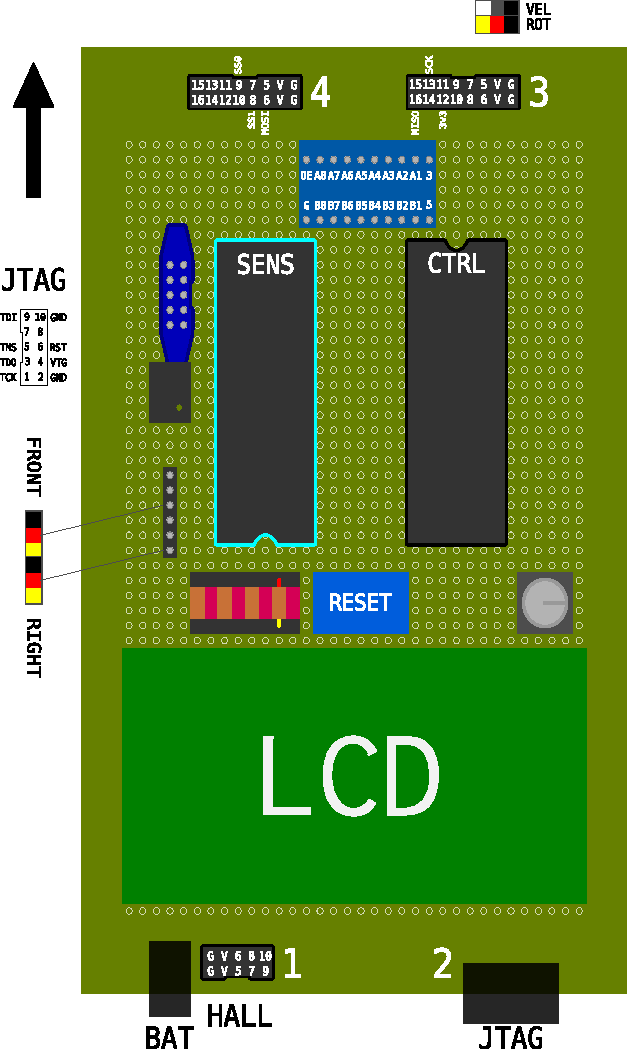
\includegraphics[width=0.6\linewidth]{\figures/kretskort-above.pdf}
    \caption{Kretskortet sedd uppifrån, jämte sensormodulen finnes en blå
    jtag-port för att flasha sensormodulen. Längst ner till höger finns
    jtag-porten för att flasha styrmodulen.}
    \label{fig:kretsabove}
\end{figure}

För flashning av moduler behöver man använda en jtag där man kopplar in usb:n i
en dator med avrdude installerat. För att flasha sensormodulen kopplar man in
jtagen i den blåa jtagporten till vänster om sensormodulen enligt bilden ovan,
sedan skriver man \mono{make sens.prog}. För att flasha styrmodulen kopplar man in
jtagen i port 2 längst ner till höger på virkortet under LCD-displayen. För att
programmera styrmodulen skriver man \mono{make ctrl.prog}.
